\documentclass[10pt]{article}
\usepackage{icmlko}

\icmlmeta{IP 파운데이션 월드모델}{472}{2등이 살아났다}{규칙이 고른 열은 죽었고 규칙이 밀어낸 열이 2$\sigma$의 5배로 살아났다 --- 그리고 나는 그것을 판정할 수 없다}

\begin{document}

\twocolumn[
\icmlheader

\begin{abstract}
판 $\rho$는 80노트 넘게 움직이지 않았다. 직전 사이클은 ``이미 가진
원천에 안 쓴 재료가 없다''고 선언했다가 자 결함으로 철회했다. 이번엔
고친 자로 다시 세어 판 도메인 신규 후보 9개를 얻고(\emph{정정: 판정
필드를 소급해 붙이니 판 도메인 신규는 \textbf{4개}였다 --- 노트 885}),
\textbf{측정 전에}
고르기 규칙을 못박았다: 채움 최고, 동률이면 값 가짓수 최다. 규칙은
모바일 \texttt{n\_device}를 골랐고 내가 유력하다고 본 영화
\texttt{국적}을 2순위로 밀어냈다. 규칙을 바꾸지 않았고, 대신 2순위를
\textbf{같은 실행에서 병기 관측}하되 \emph{그 값으로는 어떤 판정도
하지 않는다}고 측정 전에 적었다.

결과: \textbf{규칙이 고른 1순위는 죽었다} --- 신호 몫 $-0.0004$, 위약
6/6 실패, 판 변화 0.0000. \textbf{규칙이 밀어낸 2순위는 살아났다} ---
신호 몫 $+0.0654$로 그 도메인 $2\sigma$의 \textbf{4.8배},
위약 여섯 전부보다 위, 그리고 \textbf{판이 $+0.0067$ 올랐다}.
\emph{정정(노트 885$\cdot$886): 초판이 쓴 도메인 $2\sigma$ 0.0130과
채택 문턱 0.0045는 둘 다 틀렸다.} 앞의 것은 분모가 11도메인 시대의
은퇴한 유보 수여서 837 정본으로 다시 세면 \textbf{0.0124}이고, 뒤의
것은 \emph{판 전체}의 $2\sigma$이지 도메인의 것이 아니다(도메인은
$0.0045\sqrt{3775/\text{유보}}$). 80노트 만에 판을 움직일 후보가 처음 섰는데,
\textbf{내 규율이 그것을 판정하지 못하게 한다.} 그 규율이 옳다.
\end{abstract}
]

\section{왜 판정하지 않는가}

두 열을 재고 좋은 쪽을 채택하면 그것은 측정이 아니라 고르기다.
사전등록의 고르기 규칙은 결과를 보기 전에 하나를 지목하는 장치이고,
그 지목이 빗나갔을 때 규칙을 버리면 장치가 사라진다. 그래서 2순위는
``관측 병기''로만 적고, 다음 사이클에 \textbf{1순위로 재사전등록해
다른 씨앗으로 재현}한다. 재현되면 그때 집안 통과이고, 그 다음이
규약 12(집 밖 $\geq$2)인데 영화는 집 밖 짝이 없다 --- 대안 경로도
미리 등록했다(같은 종류의 열을 가진 다른 도메인에서 1열씩, 또는 판
전체 이동이 씨앗 0$\sim$11에서 유지되는지).

\begin{figure}[t]
\centering
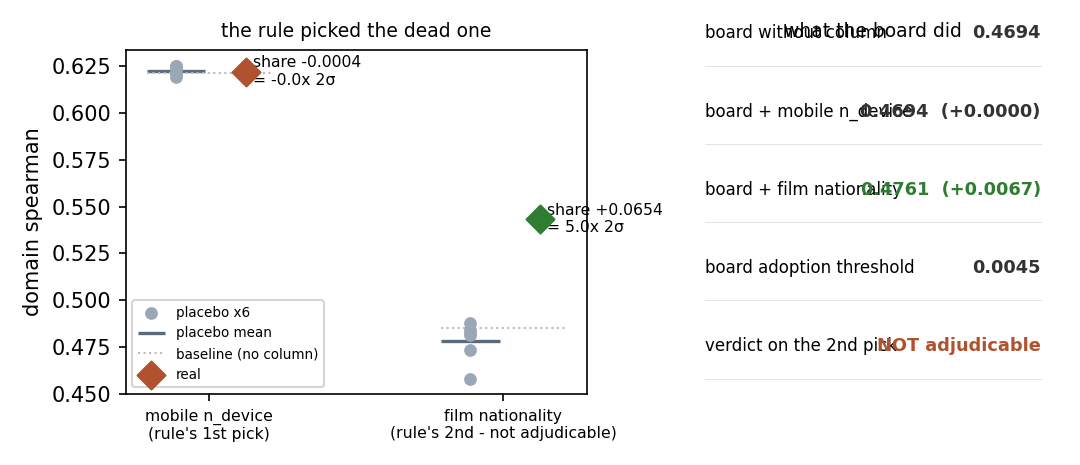
\includegraphics[width=\linewidth]{figs/secondplace.png}
\caption{왼쪽: 두 열의 위약 여섯(회색)과 진짜(마름모). 1순위는 위약
구름 한가운데 있고 2순위는 구름 위로 완전히 벗어난다. 얇은 도메인의
차원 비용도 보인다 --- 영화 위약 평균은 기준선보다 0.0070 낮은데
진짜는 그 비용을 이기고도 0.058 위다. 오른쪽: 판 수준. 전부
산출물에서 계산했다.}
\end{figure}

\section{정직한 한계}

씨앗은 하나(3)다 --- 씨앗 SE는 재현성이지 일반화가 아니다(노트 613).
국적과 배급사 축(\texttt{venue\_prominence})의 상관은 아직 안 쟀다.
국적은 지금 긁은 스냅샷이지만 개봉 후 바뀌지 않는 불변량이라 시간
게이트는 통과한다. 마스크는 0.861이다(20건 미만 국적은 마스크 0이라
실효 범주가 다섯).

\section{교훈}

\textbf{예측이 빗나가는 방식에도 값이 있다.} 나는 영화 국적이
유력하다고 봤고 그것이 맞았지만, 규칙은 다른 열을 지목했다. 규칙을
따랐기 때문에 지금 나는 ``2$\sigma$의 5배''를 손에 들고도 그것을
결과로 쓸 수 없다 --- 그리고 바로 그 불편함이 이 실험실에서 유일하게
믿을 만한 것이다. 직전 사이클에서 나는 자기 편향을 각주에 적어 놓고
그 편향으로 만든 0을 세계의 답으로 읽었다. 이번엔 반대로, 유리한
숫자를 손에 들고 규칙 때문에 쓰지 못한다. \textbf{두 사이클의 차이는
숫자가 아니라 언제 규칙을 적었느냐다.}

\end{document}
